\chapter{Legal transition binding management}\label{chapter:binding-management}

In this chapter we will discuss the major part of our project - legal transition binding management. First we will explain our algorithm to find legal transition bindings (see \nameref{section:find-bindings}).

\section{Finding legal transition bindings}\label{section:find-bindings}

In this section we will explain in details our transition binding algorithm. The algorithm starts with handling initial marking (see \nameref{subs:handling-rt}). After initial values are ready a unification (needs citing!!!) process takes place (see \nameref{subs:unification}). After unification is completed undefined variables are resolved (see \nameref{subs:resolve}). Finally, the solution is checked if it conforms to a variable definition (see \nameref{subs:check-solution}).

\subsection{Evaluating initial marking}\label{subs:handling-rt}

\begin{figure}[!htb]
  \includegraphics{img/rt-value-test.png}
  \caption{Evaluating initial marking value}\label{fig:rt-value-test}
\end{figure}

\begin{figure}[!htb]
  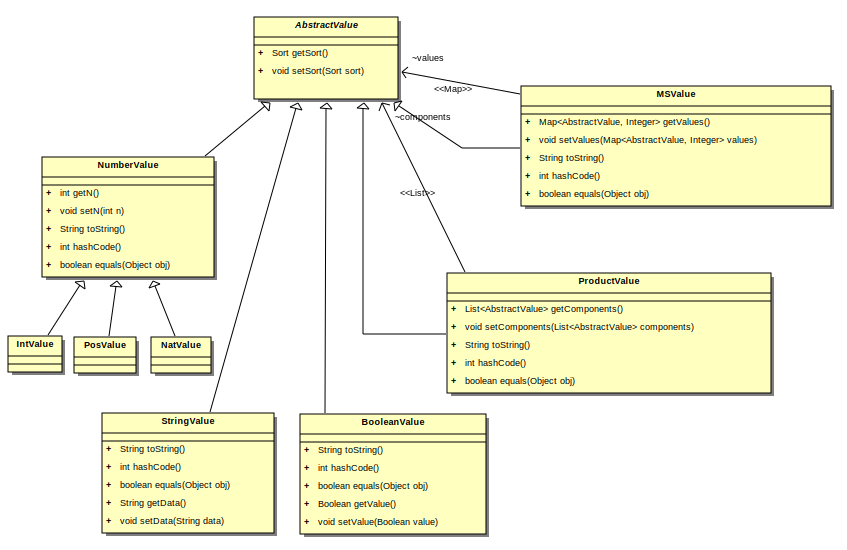
\includegraphics[scale=0.5]{img/runtime.pdf}
  \caption{Runtime value class diagram}\label{fig:rt-value}
\end{figure}

\subsection{Unification}\label{subs:unification}

Comparison is performed only on NumberOf pairs participating in multiset Add operation. In a case of subtraction only minuend is considered (subtrahend is ignored). Arc inscriptions are handled independently.

\begin{figure}[!htb]
  \includegraphics{img/unification-functions-subtract.png}
  \caption{Unification: functions and multi set subtraction}\label{fig:unification-functions-subtract}
\end{figure}

\begin{figure}[!htb]
  \includegraphics{img/unification-arithmetic.png}
  \caption{Unification: expression assignment}\label{fig:unification-arithmetic}
\end{figure}

\begin{figure}[!htb]
  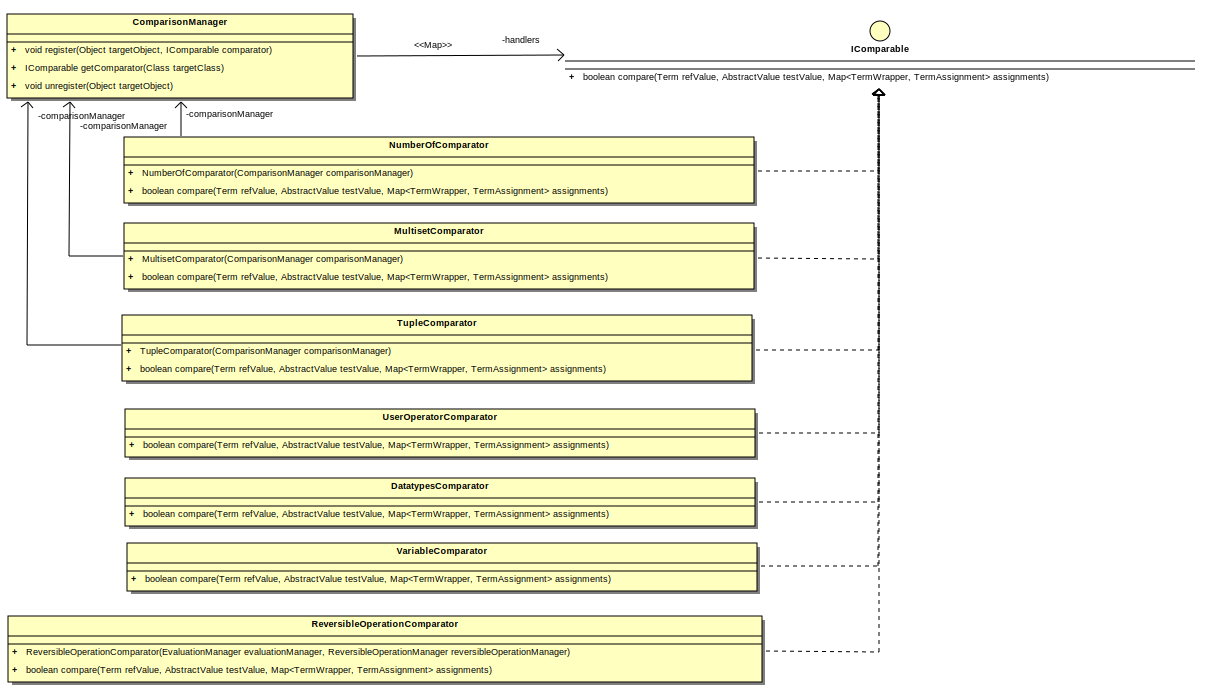
\includegraphics[scale=0.35]{img/comparators.pdf}
  \caption{Unification: comparators}\label{fig:comparators}
\end{figure}

\begin{figure}[!htb]
  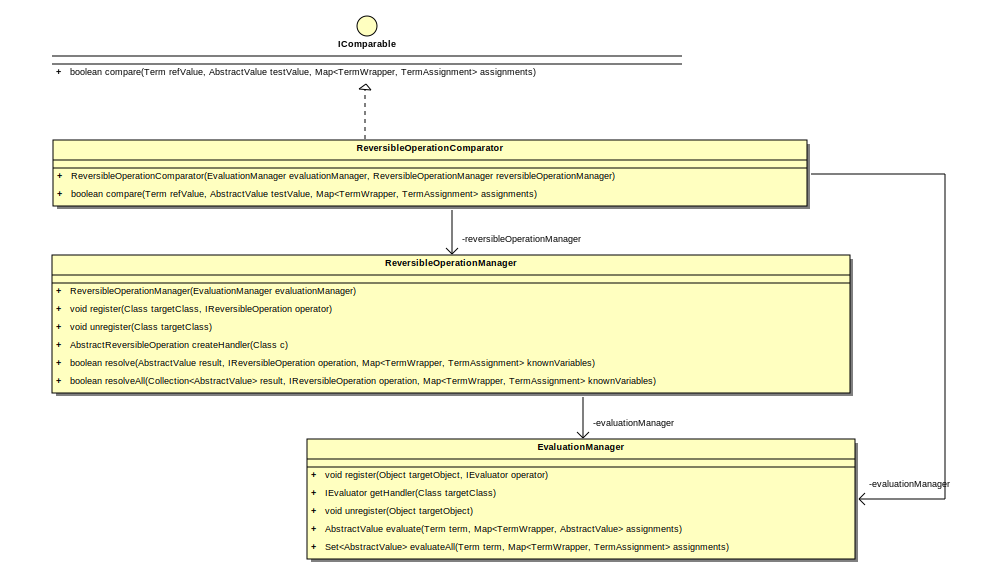
\includegraphics[scale=0.4]{img/reversibleOperationComparator.pdf}
  \caption{Unification: reversible operation comparator}\label{fig:reversible-operation-comparator}
\end{figure}

\subsection{Resolve}\label{subs:resolve}

\begin{figure}[!htb]
  \includegraphics{img/resolve.png}
  \caption{Resolve}\label{fig:resolve}
\end{figure}

\begin{figure}[!htb]
  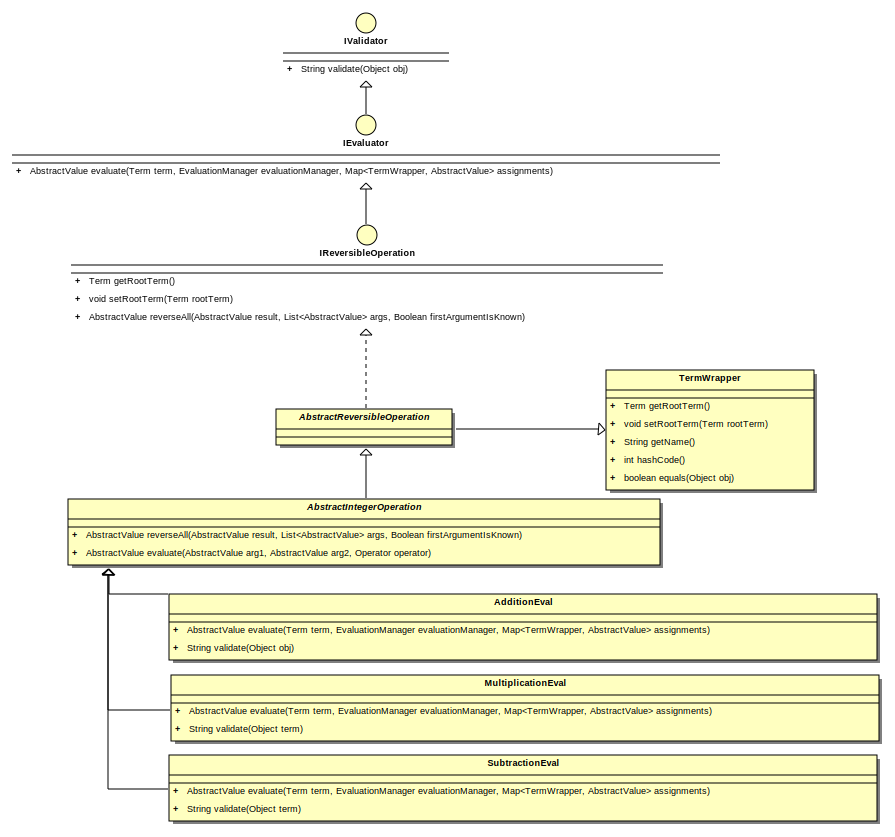
\includegraphics[scale=0.45]{img/reverseOperators.pdf}
  \caption{Unification: reversible operations}\label{fig:reverse-operators}
\end{figure}

\begin{figure}[!htb]
  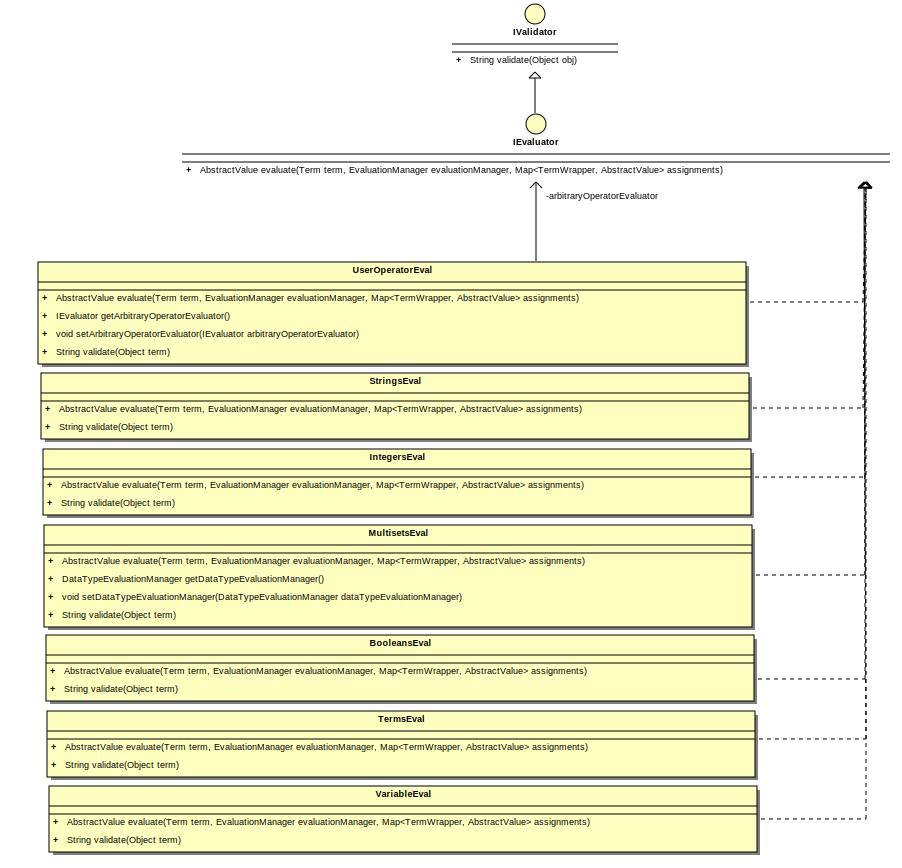
\includegraphics[scale=0.45]{img/evaluators.pdf}
  \caption{Unification: evaluators}\label{fig:evaluators}
\end{figure}

\begin{figure}[!htb]
  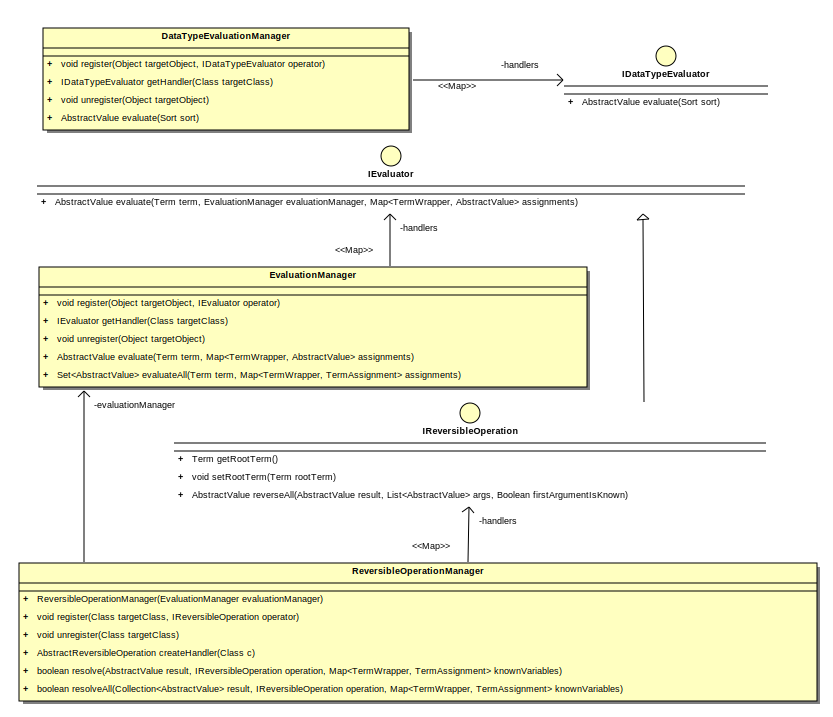
\includegraphics[scale=0.45]{img/evalManagers.pdf}
  \caption{Unification: evaluation managers}\label{fig:evalManagers}
\end{figure}

\begin{figure}[!htb]
  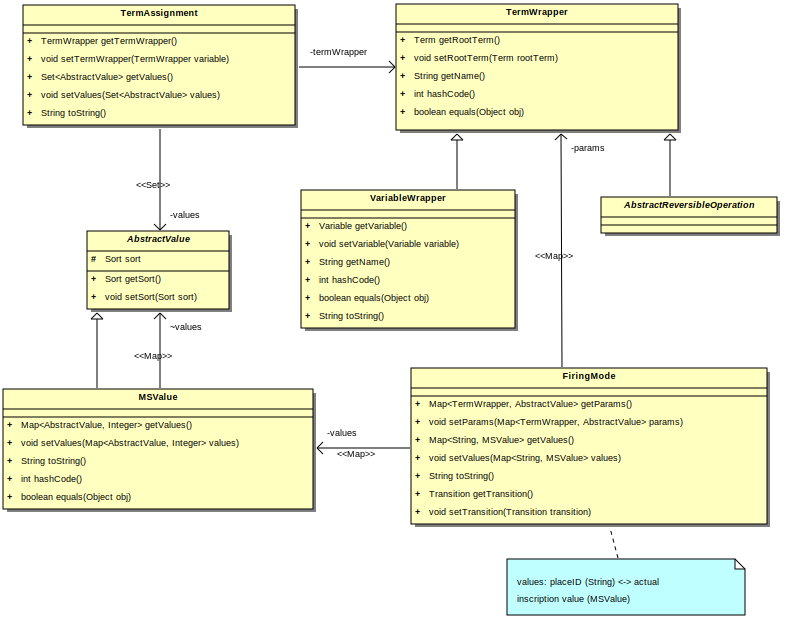
\includegraphics[scale=0.5]{img/termWrapper.pdf}
  \caption{Term wrapper}\label{fig:termWrapper}
\end{figure}

\subsection{Checking solution}\label{subs:check-solution}

\begin{figure}[!htb]
  \includegraphics[scale=0.6]{img/test19.pdf}
  \caption{A complicated technical example}\label{fig:test19}
\end{figure}
